%%% Copyright (C) 2020 David Beauchemin
%%%
%%% Ce fichier et tous les fichiers .tex dont la racine est
%%% mentionnée dans les commandes \include et \input ci-dessous font
%%% partie du projet «Gestion de la configuration et des résultats avec MLflow, Hydra et Poutyne
%%% - Webinaire»
%%% URL
%%%
%%% Le format et le visuel est très fortement inspiré du matériel de
%%% Vincent Goulet https://gitlab.com/vigou3/webinaire-recherche-reproductible
%%%
%%% Cette création est mise à disposition selon le contrat
%%% Attribution-Partage dans les mêmes conditions 4.0
%%% International de Creative Commons.
%%% https://creativecommons.org/licenses/by-sa/4.0/

\documentclass[aspectratio=169,10pt,xcolor=x11names,english,french]{beamer}
\usepackage{babel}
\usepackage[autolanguage]{numprint}
\usepackage{amsmath}
\usepackage{currfile}                  % nom fichier de script
\usepackage{changepage}                % page licence
\usepackage{tabularx}                  % page licence
\usepackage{relsize}                   % \smaller et al.
\usepackage{awesomebox}                % boites signalétiques
\usepackage{fancyvrb}                  % texte verbatim
\usepackage{framed}                    % env. leftbar
\usepackage{pict2e}                    % cycle travail Git
\usepackage[overlay,absolute]{textpos} % couvertures
\usepackage{metalogo}       
\usepackage{textpos}           % logo \XeLaTeX

\usepackage{fontawesome}

\usepackage{stackengine, tikz} % for stacking logo

\usepackage{svg} %for svg image also need option --shell-escape

\usepackage{dirtree}


%% =============================
%%  Informations de publication
%% =============================
\title{Gestion de la configuration et des résultats avec MLflow, Hydra et Poutyne}
\author{David Beauchemin}
\date{.. novembre 2020}

%% =======================
%%  Apparence du document
%% =======================

%% Couleurs additionnelles
\definecolor{rouge}{rgb}{1,0.31,0.26}
\definecolor{bleu}{rgb}{0.18,0.23,1}
\definecolor{couleurpolice}{rgb}{0.13,0.13,0.13}

\definecolor{link}{cmyk}{0.67, 0.66, 0, 0.71}    % liens internes
\definecolor{url}{rgb}{1,0.31,0.26}       % liens externes
\definecolor{codebg}{rgb}{0.94, 0.95, 0.95}

\colorlet{shadecolor}{codebg}

%% Thème Beamer général
\usetheme[titleformat=allcaps, numbering=none, block=transparent]{metropolis}

%% Modifications aux couleurs: fond blanc, titres en texte noir sur
%% fond blanc
\setbeamercolor{normal text}{bg=white}
\setbeamercolor{frametitle}{fg=normal text.fg, bg=}

%% Déplacer les titres vers le bas sous la décoration du gabarit CFDD
\makeatletter
\setlength{\metropolis@frametitle@padding}{4.9ex}
\renewcommand{\metropolis@frametitlestrut@start}{
	\rule{0pt}{6ex +%
		\totalheightof{%
			\ifcsdef{metropolis@frametitleformat}{\metropolis@frametitleformat X}{X}%
		}%
	}
}
\renewcommand{\metropolis@frametitlestrut@end}{}
\makeatother

%% Format de la page de titre de section;
\makeatletter

\setbeamertemplate{section page}{%
	\begin{minipage}{22em}
		\raggedright
		\usebeamerfont{section title}
		\let\hyperlink\@secondoftwo\fontsize{35}{35}\textcolor[cmyk]{0.67, 0.66, 0, 0.71}{\insertsectionhead}\par
	\end{minipage}
	\par
	\vspace{\baselineskip}
}

\makeatother

%% Polices de caractères
\newfontfamily\Overpass{Overpass}
\setsansfont{Overpass}        % police principale
\newfontfamily\OverpassSemiBold{Overpass}
[
BoldFont = *-SemiBold
]
\newfontfamily\OverpassExtraLightBold{Overpass}
[
UprightFont = *-ExtraLight,
BoldFont = *-Light
]
\newfontfamily\OverpassLight{Overpass}
[
UprightFont = *-Light,
BoldFont = *-Regular
]


\setbeamercolor{frametitle}{fg=couleurpolice}
\setbeamercolor{section in head/foot}{fg=couleurpolice}
\setbeamercolor{normal text}{fg=couleurpolice}



%% Hyperliens
\hypersetup{%
	pdfauthor = {David Beauchemin},
	pdftitle = {Gestion de la configuration et des résultats avec MLflow, Hydra et Poutyne},
	colorlinks = {true},
	linktocpage = {true},
	allcolors = {link},
	urlcolor = {url},
	pdfpagemode = {UseOutlines},
	pdfstartview = {Fit},
	bookmarksopen = {true},
	bookmarksnumbered = {true},
	bookmarksdepth = {subsection}}

%% Paramétrage de babel pour les guillemets
\frenchbsetup{og=«, fg=»}

%% =========================
%%  Nouveaux environnements
%% =========================

%% Environnement pour le code informatique; hybride
%% des environnements snugshade* et leftbar de framed.
\makeatletter
\newenvironment{Scode}{%
	\def\FrameCommand##1{\hskip\@totalleftmargin
		\vrule width 3pt\colorbox{codebg}{\hspace{5pt}##1}%
		% There is no \@totalrightmargin, so:
		\hskip-\linewidth \hskip-\@totalleftmargin \hskip\columnwidth}%
	\MakeFramed {\advance\hsize-\width
		\@totalleftmargin\z@ \linewidth\hsize
		\advance\labelsep\fboxsep
		\@setminipage}%
}{\par\unskip\@minipagefalse\endMakeFramed}
\makeatother

%% Environnement pour le contenu d'un fichier; alias de snugshade*.
\newenvironment{Sfile}{\begin{snugshade*}}{\end{snugshade*}}

%% =====================
%%  Nouvelles commandes
%% =====================

%% Lien externe
\newcommand{\link}[2]{\href{#1}{#2~{\smaller\faExternalLink*}}}
\newcommand{\guillemet}[1]{\guillemotleft #1 \guillemotright}

%% Simili commande \HUGE
\newcommand{\HUGE}{\fontsize{36}{36}\selectfont}

%%% =======
%%%  Varia
%%% =======

%% Longueurs pour la composition des pages couvertures avant et
%% arrière
\newlength{\banderougewidth} \newlength{\banderougeheight}
\newlength{\bandeorwidth}    \newlength{\bandeorheight}
\newlength{\imageheight}     \newlength{\imagewidth}
\newlength{\logoheight}

\begin{document}
	
	%% Style de l'entête et du pied de page
	
	%% frontmatter
	%%% Copyright (C) 2020 David Beauchemin
%%%
%%% Ce fichier et tous les fichiers .tex dont la racine est
%%% mentionnée dans les commandes \include et \input ci-dessous font
%%% partie du projet Gestion de la configuration et des résultats avec MLflow, Hydra et Poutyne
%%% - Webinaire»
%%% URL
%%%
%%% Le format et le visuel est très fortement inspiré du matériel de
%%% Vincent Goulet https://gitlab.com/vigou3/webinaire-recherche-reproductible
%%%
%%% Cette création est mise à disposition selon le contrat
%%% Attribution-Partage dans les mêmes conditions 4.0
%%% International de Creative Commons.
%%% https://creativecommons.org/licenses/by-sa/4.0/

%% Normes de présentation visuelle 2018
%%
%% - grille de 8 unités de haut
%% - 1 mesure = 1/8 d'unité
%% - bande identitaire de 1 mesure placée au bas de la 7e unité
%% - logo haut de 4 mesures avec blancs de deux mesures en haut et
%%   en bas
%% - blanc équivalent à la largeur du blason à droite du logo
%% - bande or de la largeur du logo + blanc à droite
%%
%% Dimensions du logo UL
%%
%% hauteur: 129
%% largeur totale: 312
%% largeur blason: 102
%% valeur clé: (312 + 102)/129 = 3.209302
%%
%% Dimensions de l'image
%%
%% hauteur: 55 mesures - 1pt (filet) = 54.9191919 mesures
%% largeur: 160mm
%% ratio largeur/hauteur: 160/77.23

\begingroup
\TPGrid{16}{64}
\textblockorigin{0mm}{0mm}
\setlength{\parindent}{0mm}
\setlength{\imageheight}{54.9191919\TPVertModule}
\setlength{\logoheight}{4\TPVertModule}
\setlength{\bandeorwidth}{3.209302\logoheight}
\setlength{\banderougewidth}{\paperwidth}
\addtolength{\banderougewidth}{-\bandeorwidth}
\setlength{\bandeorheight}{\TPVertModule}
\setlength{\banderougeheight}{\TPVertModule}
\setlength{\textwidth}{\paperwidth}
\addtolength{\textwidth}{-2\TPHorizModule}

\def\titlefmt{%
  \bfseries\fontsize{19}{19}\selectfont%
  CONFIGURATION AND RESULTS MANAGEMENT WITH MLFLOW, HYDRA ET POUTYNE\par}
\def\webinaire{%
  \OverpassSemiBold\bfseries\fontsize{18}{18}\selectfont
  SEMINAR}
\def\datefmt{%
  \OverpassExtraLightBold\bfseries\fontsize{14}{14}\selectfont%
  JANUARY 19, 2021}

%%%
%%% Page de titre
%%%
\begin{frame}[plain]
  %% bandeau identitaire
  \begin{textblock*}{\paperwidth}[0,1](0mm,56\TPVertModule)
    \textcolor{rouge}{\rule{\banderougewidth}{\banderougeheight}}%
    \textcolor{bleu}{\rule{\bandeorwidth}{\bandeorheight}}
  \end{textblock*}

  %% identifiant «webinaire»
  \begin{textblock*}{2\TPHorizModule}(0.7\TPHorizModule,5\TPVertModule)
    \textcolor[rgb]{0.13,0.13,0.13}{\webinaire}
  \end{textblock*}

  %% titre
  \begin{textblock*}{12\TPHorizModule}(0.7\TPHorizModule,17\TPVertModule)
    \textcolor[rgb]{0.13,0.13,0.13}{\titlefmt}
  \end{textblock*}

  %% date
  \begin{textblock*}{10\TPHorizModule}(0.7\TPHorizModule,41\TPVertModule)
    \textcolor[rgb]{0.13,0.13,0.13}{\datefmt}
  \end{textblock*}
\end{frame}
\endgroup

	
	\begin{frame}{Objectifs de la présentation}
		\begin{itemize}
			\item Initier aux outils de gestion de l'entrainement, de la configuration et des résultats.
			\item Développer de bonnes pratiques.
			\item Améliorer votre productivité.
		\end{itemize}
	\end{frame}
	
	\begin{frame}
		\frametitle{Votre conférencier}
		
		\begin{minipage}{0.25\linewidth}
			
\includegraphics[width=\linewidth,keepaspectratio]{img/david}
		\end{minipage}
		\hfill
		\begin{minipage}{0.70\linewidth}
			\begin{itemize}
				\item Introduit à la recherche reproductible en 2016 (\mbox{R Markdown} et \faGit)
				\item Participation à REPROLANG de la conférence LREC \cite{garneau2020robust}
				\item Membre actif dans le développement d'une librairie facilitant la reproductibilité (\link{https://poutyne.org/}{Poutyne})
			\end{itemize}
		\end{minipage}
		
		\begin{minipage}{0.25\linewidth}
			\small
			\textbf{DAVID BEAUCHEMIN} \\
			Candidat au doctorat \\
			Département d'informatique et de génie logiciel
		\end{minipage}
	\end{frame}

	\begin{frame}{Au menu}
		\begin{minipage}{0.49\linewidth}
				\centering
				\fontsize{35}{35}\faCog\vfil
				\vspace{1em}
				\normalsize Gestion de la configuration
				
		\end{minipage}
		\begin{minipage}{0.49\linewidth}
				\centering
				\fontsize{35}{35}\faAreaChart\vfil
				\vspace{1em}
				\normalsize Gestion des résultats
		\end{minipage}
	\end{frame}
	
	\section{La gestion d'un projet}
	\begin{frame}{Gestion des paramètres de configuration}
		\begin{Scode}
			@experiment.config \\
			def config(): \\
			\quad	seed = 42 \\
			\quad	num\_runs = 10 \\
			\quad	iteration = 0 \\
			\quad	source\_language = "en" \\
			\quad	target\_language = "de" \\
			\quad 	src\_input = "path"  \# The input source embeddings \\
			\quad 	trg\_input = "2e path" \# The input target embeddings \\
			\quad 	other\_input = "3e path" \# Commentaire pas clair \\
			\quad   $\vdots$ \\
			\quad   (ligne 500) $n^e$ paramètre \\
		\end{Scode}
	\end{frame}

	\begin{frame}{Gestion des paramètres de configuration}
		\centering
		\uncover<1->{\begin{minipage}{0.24\linewidth}
				\centering
				\normalsize Quel paramètre fait ça déjà?
		\end{minipage}}
		\uncover<2->{\begin{minipage}{0.24\linewidth}
				\centering
				\normalsize Quels paramètres sont nécessairement ensemble?
		\end{minipage}}
		\uncover<3->{\begin{minipage}{0.24\linewidth}
				\centering
				\normalsize Sont-ils tous essentiels?
		\end{minipage}}
		\uncover<4->{\begin{minipage}{0.24\linewidth}
				\centering
				\normalsize Comment doit-on se retrouver dans le projet?
		\end{minipage}}
	\end{frame}

	\begin{frame}{Gestion des résultats}
		\begin{Scode}
			\dirtree{%
			.1 .
			.2 res\_1.txt.
			.2 res\_2.txt.
			.2 res\_3.txt.
			.2 res\_4.txt.
			.2 res\_5\_good.txt.
			.2 res\_5.txt.
			.2 res\_6\_fix\_a.txt.
			.2 $\vdots$.
			.2 $n^e$ fichier de résultats.
		}
		\end{Scode}
	\end{frame}

	\begin{frame}{Gestion des résultats}
		\centering
		\uncover<1->{\begin{minipage}{0.24\linewidth}
				\centering
				\normalsize Quelle configuration déjà avec ces résultats?
		\end{minipage}}
		\uncover<2->{\begin{minipage}{0.24\linewidth}
				\centering
				\normalsize Est-ce un succès ou un échec cet entrainement?
		\end{minipage}}
		\uncover<3->{\begin{minipage}{0.24\linewidth}
				\centering
				\normalsize Lequel contient mes meilleurs résultats?
		\end{minipage}}
		\uncover<4->{\begin{minipage}{0.24\linewidth}
				\centering
				\normalsize Comment doit-on se retrouver dans les résultats?
		\end{minipage}}
	\end{frame}

	
	\section{Les solutions}
	
	\begin{frame}{Au menu}
		\begin{minipage}{0.49\linewidth}
			\centering
			\fontsize{35}{35}\faCog
			\vfil
			\vspace{1em}
			\normalsize Gestion de la configuration
			
		\end{minipage}
		\begin{minipage}{0.49\linewidth}
			\centering
			\tikz\node[opacity=0.5]{\fontsize{35}{35}\faAreaChart};
			\vfil
			\vspace{1em}
			\tikz\node[opacity=0.5]{\normalsize Gestion des résultats};
		\end{minipage}
	\end{frame}

	\begin{frame}{Gestion de la configuration}
		\centering
		\uncover<1->{\begin{minipage}{0.32\linewidth}
				\centering
				\fontsize{35}{35}\faForward\vfil
				\vspace{1em}
				\normalsize Simple et efficace
		\end{minipage}}
		\uncover<2->{\begin{minipage}{0.32\linewidth}
				\centering
				\fontsize{35}{35}\faFlask\vfil
				\vspace{1em}
				\normalsize Facilite l'expérimentation
		\end{minipage}}
		\uncover<3->{\begin{minipage}{0.32\linewidth}
				\centering
				\fontsize{35}{35}\faLineChart\vfil
				\vspace{1em}
				\normalsize Extensible
		\end{minipage}}
		\note{
			On cherche une solution qui va être :
			
			simple et efficace pour gérer nos configurations,
			
			qui va faciliter l'expérimentation plutôt que la ralentir,
			
			extensible pour permettre la définition de plusieurs paramètres tout en étant concis.
		}
		
	\end{frame}
	
	\begin{frame}
		\frametitle{\link{https://hydra.cc/}{Hydra}}
		\framesubtitle{\textit{A framework for elegantly configuring complex applications}}
		
		\centering
		\begin{minipage}{0.24\linewidth}
				\centering
				\fontsize{35}{35}\faIcon{osi}\vfil
				\vspace{1em}
				\normalsize \textit{Open source} et licence MIT
		\end{minipage}
		\begin{minipage}{0.24\linewidth}
				\centering
				\fontsize{35}{35}\faFile\vfil
				\vspace{1em}
				\normalsize Fichiers de configurations structurés YAML
		\end{minipage}
		\begin{minipage}{0.24\linewidth}
				\centering
				\fontsize{35}{35}\faIcon{cubes}\vfil
				\vspace{1em}
				\normalsize Fichiers de configurations hiérarchiques
		\end{minipage}
		\begin{minipage}{0.24\linewidth}
			\centering
			\fontsize{35}{35}\faCogs\vfil
			\vspace{1em}
			\normalsize Balayage de configurations
		\end{minipage}
		\note{
		}
	\end{frame}
	
	\begin{frame}{Configuration structuré}
		\begin{Scode}
			\dirtree{%
				.1 conf.
				.2 config.yaml.
				.2 dataset.
				.3 canadian.yaml.
				.3 netherlands.yaml.
				.2 embeddings.
				.3 fast\_text.yaml.
				.2 model.
				.3 bi\_lstm\_bidirectionnal.yaml.
				.3 bi\_lstm.yaml.
				.3 lstm\_bidirectionnal.yaml.
				.3 lstm.yaml.
				.2 optimizer.
				.3 adam.yaml.
				.3 SGD.yaml.
			}
		\end{Scode}
	\end{frame}

	\begin{frame}{Configuration hiérarchique}
		\begin{Scode}
			data\_loader: \\
			\quad	batch\_size: 2048 \\
			setting: \\
			\quad seed: 42 \\
			\quad device: "cuda:0" \\
			defaults: \\
			\quad - optimizer: SGD \\
			\quad - model: bi\_lstm \\
			\quad - dataset: canadian \\
			\quad - embeddings: fast\_text \\
			trainer: \\
			\quad num\_epochs: 1 \\
			\quad patience: 30 \\
		\end{Scode}
	\end{frame}

	\begin{frame}{Configuration hiérarchique}
		optimizer: SGD
		\begin{Scode}
			optimizer: \\
			\quad lr: 0.1 \\
			\quad type: sgd \\
		\end{Scode}
	\end{frame}

	\begin{frame}{Balayage de configurations}
			
			\begin{Scode}
				python main.py --multirun task=1,2,3,4,5
			\end{Scode}
			
			\begin{Scode}
				python main.py -m 'main.x=int(interval(-5, 5))' 'main.y=interval(-5, 10)'
			\end{Scode}
		\note{Plusieurs choix de sweeper Ax, Joblib, Nevergrad}
	\end{frame}

	\begin{frame}{En bonus}
		\begin{itemize}
			\item Journalisation automatique et personnalisable
			\item Instanciation paramétrique 
			\begin{Scode}
				\# @package \_group\_ \\
				\quad \_target\_: my\_app.MySQLConnection \\
				\quad host: localhost \\
				\quad user: root \\
				\quad password: 1234 \\
			\end{Scode}
		\end{itemize}
	\end{frame}

	\begin{frame}{Point négatif}
		\begin{Scode}
			hydra.utils.get\_original\_cwd()
		\end{Scode}
	\note{En raison de la journalisation automatique, le working directory change.}
	\end{frame}

	\begin{frame}{Au menu}
		\begin{minipage}{0.49\linewidth}
			\centering
			\tikz\node[opacity=0.5]{\fontsize{35}{35}\faCog};
			\vfil
			\vspace{1em}
			\tikz\node[opacity=0.5]{\normalsize Gestion de la configuration};
			
		\end{minipage}
		\begin{minipage}{0.49\linewidth}
			\centering
			\fontsize{35}{35}\faAreaChart
			\vfil
			\vspace{1em}
			\normalsize Gestion des résultats
		\end{minipage}
	\end{frame}

	\begin{frame}{Gestion des résultats}
	\centering
	\uncover<1->{\begin{minipage}{0.32\linewidth}
			\centering
			\fontsize{35}{35}\faIcon{user-check}\vfil
			\vspace{1em}
			\normalsize Simple à utiliser
	\end{minipage}}
	\uncover<2->{\begin{minipage}{0.32\linewidth}
			\centering
			\fontsize{35}{35}\faIcon{archive}\vfil
			\vspace{1em}
			\normalsize Journalisation des expérimentations
	\end{minipage}}
	\uncover<3->{\begin{minipage}{0.32\linewidth}
			\centering
			\fontsize{35}{35}\faLineChart\vfil
			\vspace{1em}
			\normalsize Visualisation rapide des expérimentations
	\end{minipage}}
	\note{
		On cherche une solution qui va être :
		
		simple à utiliser et \textit{utilisateur ready},
		
		qui va journaliser \textbf{intelligemment} nos expérimentations,
		
		qui permet de visualiser rapidement nos expérimentations et les comparer.
	}
	\end{frame}

	\begin{frame}
		\frametitle{\link{https://mlflow.org/}{MLflow Tracking}}
		\framesubtitle{\textit{An open source platform for the machine learning lifecycle}}
		
		\centering
		\begin{minipage}{0.24\linewidth}
			\centering
			\fontsize{35}{35}\faIcon{osi}\vfil
			\vspace{1em}
			\normalsize \textit{Open source} et licence Apache 2.0
		\end{minipage}
		\begin{minipage}{0.24\linewidth}
			\centering
			\fontsize{35}{35}\faIcon{cogs}\vfil
			\vspace{1em}
			\normalsize Suivie automatique de paramètres d'entrainement
		\end{minipage}
		\begin{minipage}{0.24\linewidth}
			\centering
			\fontsize{35}{35}\faLineChart\vfil
			\vspace{1em}
			\normalsize Visualisation simple
		\end{minipage}	
		\begin{minipage}{0.24\linewidth}
			\centering
			\fontsize{35}{35}\faIcon{cubes}\vfil
			\vspace{1em}
			\normalsize Intégration avec Poutyne
		\end{minipage}
		\note{
		}
	\end{frame}

	\begin{frame}{Suivie automatique de paramètres d'entrainement}
		\begin{itemize}
			\item Version du code (\faGit)*
			\item Horodatage de l'entrainement
			\item Succès/échec de l'entrainement
			\item Configuration de l'ordinateur
			\item Utilisateur
		\end{itemize}
	\note{*lorsque l'on utilise MLflow project}
	\end{frame}

	\begin{frame}{Visualisation simple}
		\begin{Scode}
			mlflow server -p 5000 -h 127.0.0.1 --backend-store-uri file:///absolute/path
		\end{Scode}
		\note{--backend-store-uri permet de gérer le lieu de la persistance
		-h 127.0.0.1 permet d'ouvrir le port sinon 0.0.0.0 pour un local}
	\end{frame}

	\begin{frame}{Visualisation simple}
		\centering
		\begin{figure}
			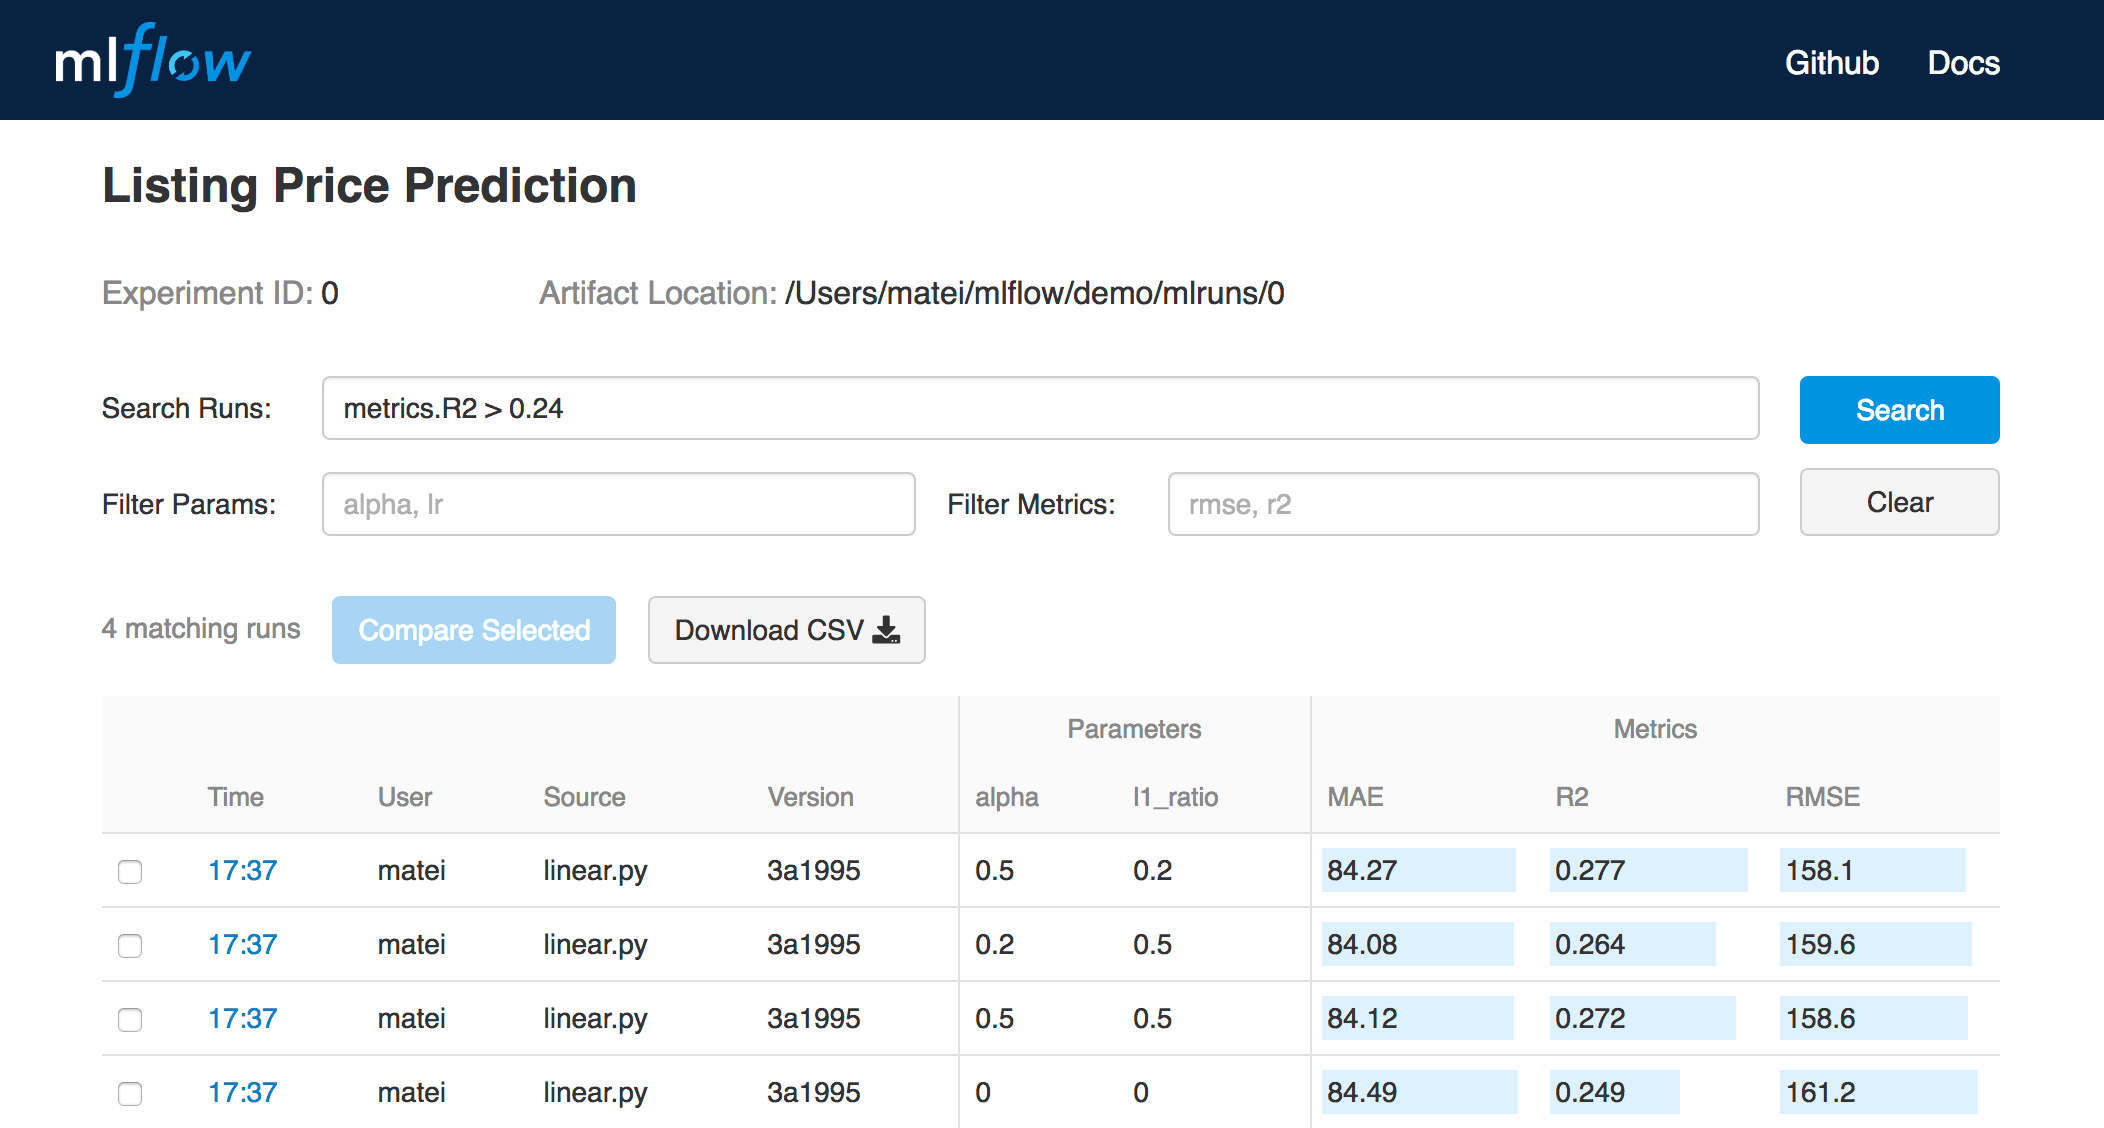
\includegraphics[width=\linewidth,keepaspectratio, height=0.7\textheight]{img/mlflow-ui.png}
			\caption{\link{https://databricks.com/blog/2018/06/05/introducing-mlflow-an-open-source-machine-learning-platform.html}{Introducing MLflow: an Open Source Machine Learning Platform}}
		\end{figure}
	\end{frame}

	\begin{frame}{Visualisation simple}
		\begin{itemize}
			\item Tri sur les expérimentations
			\item Recherche des expérimentations
			\item Requêtes sur les résultats
			\item Exportation des résultats
			\item Visualisation les métriques
		\end{itemize}
	\end{frame}


	\begin{frame}{Intégration avec \link{https://poutyne.org/}{Poutyne}}
		La version de \guillemet{base} implique de
		\begin{itemize}
			\item journaliser manuellement les paramètres de configuration,
			\item journaliser manuellement les métriques à chaque étape et itération,
			\item journaliser manuellement la version du code.
		\end{itemize}
	\end{frame}

	\begin{frame}{Intégration avec \link{https://poutyne.org/}{Poutyne}}
		La solution, \color{bleu}MLFlowWriter\color{couleurpolice}, un \textit{callback} permettant de
		\begin{itemize}
			\item journaliser semi-automatiquement les paramètres de configuration,
			\item journaliser automatiquement les métriques à chaque étape et itération,
			\item journaliser automatiquement la version du code,
			\item journaliser manuellement un modèle,
			\item journaliser automatiquement les métriques de test lors d'une phase de test.
		\end{itemize}
	\end{frame}

	\begin{frame}{Point négatif}
		La documentation n'est pas toujours facile à naviguer.
	\end{frame}

		
	\section{La suite}
	\begin{frame}{Présentation des résultats}
				\centering
		\begin{minipage}{0.49\linewidth}
				\centering
				\fontsize{35}{35}\faTable\vfil
				\vspace{1em}
				\normalsize Génération automatique des tableaux
		\end{minipage}
		\begin{minipage}{0.49\linewidth}
				\centering
				\fontsize{35}{35}\faIcon{react}\vfil
				\vspace{1em}
				\normalsize Rapport dynamique
		\end{minipage}
	\end{frame}
	\begin{frame}
		\centering
		\fontsize{35}{35}\faRefresh\vfil
		\vspace{1em}
		\normalsize Itérations d'expérimentations
		\note{Développer des processus rigoureux (par essais, erreurs et journaux) et ne pas prendre tout ce qui a été discuté ici comme l'unique solution.}
	\end{frame}
	
	\begin{frame}{Pour aller plus loin (en ordre)}
		\begin{itemize}
			\item Notification de l'état d'entrainement \link{https://notificationdoc.ca/}{Notif}
			\item \link{https://cml.dev/}{Continuous Machine Learning (CML)} 
		\end{itemize}
	\end{frame}
	
	\begin{frame}
		\frametitle{Période de questions}
		
		\centering
		\fontsize{100}{100}
		\faQuestion
		
	\end{frame}

	%%% Copyright (C) 2020 David Beauchemin
%%%
%%% Ce fichier et tous les fichiers .tex dont la racine est
%%% mentionnée dans les commandes \include et \input ci-dessous font
%%% partie du projet Gestion de la configuration et des résultats avec MLflow, Hydra et Poutyne
%%% - Webinaire»
%%% URL
%%%
%%% Le format et le visuel est très fortement inspiré du matériel de
%%% Vincent Goulet https://gitlab.com/vigou3/webinaire-recherche-reproductible
%%%
%%% Cette création est mise à disposition selon le contrat
%%% Attribution-Partage dans les mêmes conditions 4.0
%%% International de Creative Commons.
%%% https://creativecommons.org/licenses/by-sa/4.0/

%% Normes de présentation visuelle 2018
%%
%% - grille de 8 unités de haut
%% - 1 mesure = 1/8 d'unité
%% - bande identitaire de 1 mesure placée au bas de la 7e unité
%% - logo haut de 4 mesures avec blancs de deux mesures en haut et
%%   en bas
%% - blanc équivalent à la largeur du blason à droite du logo
%% - bande or de la largeur du logo + blanc à droite
%%
%% Dimensions du logo UL
%%
%% hauteur: 129
%% largeur totale: 312
%% largeur blason: 102
%% valeur clé: (312 + 102)/129 = 3.209302
%%
%% Dimensions de l'image
%%
%% hauteur: 55 mesures - 1pt (filet) = 54.9191919 mesures
%% largeur: 160mm
%% ratio largeur/hauteur: 160/77.23

\begingroup
\TPGrid{16}{64}
\textblockorigin{0mm}{0mm}
\setlength{\parindent}{0mm}
\setlength{\imageheight}{54.9191919\TPVertModule}
\setlength{\logoheight}{4\TPVertModule}
\setlength{\bandeorwidth}{3.209302\logoheight}
\setlength{\banderougewidth}{\paperwidth}
\addtolength{\banderougewidth}{-\bandeorwidth}
\setlength{\bandeorheight}{\TPVertModule}
\setlength{\banderougeheight}{\TPVertModule}
\setlength{\textwidth}{\paperwidth}
\addtolength{\textwidth}{-2\TPHorizModule}

\def\titlefmt{%
  \bfseries\fontsize{24}{24}\selectfont%
  THANK YOU FOR \\ LISTENING!\par}
\def\webinaire{%
  \OverpassSemiBold\bfseries\fontsize{18}{18}\selectfont
  SEMINAR}

%%%
%%% Page de titre
%%%
\begin{frame}[plain]
  %% bandeau identitaire
  \begin{textblock*}{\paperwidth}[0,1](0mm,56\TPVertModule)
    \textcolor{rouge}{\rule{\banderougewidth}{\banderougeheight}}% % bande rouge
    \textcolor{bleu}{\rule{\bandeorwidth}{\bandeorheight}}           % bande or
  \end{textblock*}

  %% identifiant «webinaire»
	\begin{textblock*}{2\TPHorizModule}(0.7\TPHorizModule,5\TPVertModule)
		\textcolor[rgb]{0.13,0.13,0.13}{\webinaire}
	\end{textblock*}

  %% titre
  \begin{textblock*}{12\TPHorizModule}(0.7\TPHorizModule,17\TPVertModule)
	\textcolor[rgb]{0.13,0.13,0.13}{\titlefmt}
	\end{textblock*}
\end{frame}

\endgroup

%%% Local Variables:
%%% mode: latex
%%% TeX-engine: xetex
%%% TeX-master: "webinaire-recherche-reproductible"
%%% End:

	
	\begin{frame}[t, allowframebreaks]
		\frametitle{References}
		\bibliographystyle{apalike}
		\bibliography{GECR}
	\end{frame}
	
	
	
\end{document}
